\documentclass[geye,black,normal,cn]{elegantnote}

\title{\bfseries ElegantNote:一个优美的 \LaTeX{} 笔记模板}

\author{\href{https://ddswhu.me/}{\itshape 邓东升} \\
		Elegant\LaTeX{} Group	\thanks{Elegant\LaTeX{} 其他模板下载地址:\href{https://ddswhu.me/resource/}{https://ddswhu.me/resource/}} }
\date{\small\itshape 版本:2.00 \\ 更新时间:\today}

\usepackage{listings} 
\lstset{language=[LaTeX]{TeX},basicstyle=\footnotesize\ttfamily}


\begin{document}
{\color{ecolor}{\maketitle}}
% logo
\centerline{
\includegraphics[width=0.25\textwidth]{ElegantLaTeX_green.pdf}}

\section{模板设计}
此模板设计的初衷是为了记录笔记,在 2013 年开始构想,初版我们设计了非常美观的定理环境,并设计了 3 套不同的颜色主题。但我们发现在实际记笔记的时候,过多的定理区块使得整个文章并不是非常美观,所以我们把 ElegantNote 更新为 ElegantBook 模板,在后面被用户熟知。而 ElegantNote 的设计自此停止。

2018 年,在被一些用户“催更”之后,ElegantBook 迎来重大更新,原先浮动的定理环境用 tcolorbox 全部改写。时至今日,ElegantBook 版本为 3.02。之后,我们便想把 ElegantNote 也彻底更新下,放弃 ElegantBook 中的定理环境设计,改用更为紧凑,更加朴素的定理环境,设计更适合笔记记录和笔记阅读的 \LaTeX{} 模板。

在一些朋友的建议和启发下,我们基于标准的 \LaTeX{} 文类 article 重新设计了新版 ElegantNote 模板,在此特别感谢!新模板有下面几个特性:
\begin{itemize}
\item 添加护眼模式,颜色为绿豆沙颜色;
\item 适配不同设备,包括 Pad(默认),Kindle,PC(双页),通用(A4);
\item 5 套颜色主题,分别是:green(默认),cyan,blue,sakura,black;
\item 语言模式支持:中文(默认),英文;
\item 支持 pdflatex 和 xelatex 编译;
\item 更加美观的图表标题格式,列表环境,数学字体等。
\end{itemize}

\subsection{护眼模式}
本模板增加了护眼模式,默认为不开启,开启的方法如下(2 选 1):
\begin{lstlisting}[frame=none]  
\documentclass[geye]{elegantnote}
\documentclass[mode=geye]{elegantnote}
\end{lstlisting}

\begin{remark}
此次更新只添加了护眼模式,也即只添加了一个背景颜色,如果您有希望增加其他颜色,可以和我们反馈!
\end{remark}

\subsection{设备选择}
本模板适配不同的屏幕大小,分别为 Pad,Kindle,PC,A4。不同屏幕的选择为
\begin{lstlisting}[frame=none]  
\documentclass[device=pad]{elegantnote}
\documentclass[device=kindle]{elegantnote}
\documentclass[device=pc]{elegantnote}
\documentclass[device=normal]{elegantnote}
\end{lstlisting}
\begin{note}
也可以采取直接赋值的方法选择屏幕,比如:
\end{note}
\begin{lstlisting}[frame=none]  
\documentclass[pad]{elegantnote}
\end{lstlisting}

需要注意的是,如果想要得到普通的 A4 纸张大小的 PDF,需要选择 \lstinline{device=normal},而不是选择 \lstinline{device=pc},因为  \lstinline{devic=pc} 实际上设置的是电脑双页模式。

\subsection{颜色主题}
本模板内置 5 套颜色主题,分别是 green,cyan,blue,sakura,black。其中 green 为默认颜色主题,如果用户不需要彩色,可以选择 black 主题。颜色主题的启用方法和之前一样:
\begin{lstlisting}[frame=none]  
\documentclass[green]{elegantnote}
\documentclass[color=green]{elegantnote}
\end{lstlisting}

\subsection{语言模式}
本模板内含两套语言环境,改变语言环境会改变图表标题的引导词(图,表),文章结构词(比如目录,参考文献等),以及定理环境中的引导词(比如定理,引理等)。不同语言模式的启用如下:
\begin{lstlisting}[frame=none]  
\documentclass[cn]{elegantnote}
\documentclass[lang=cn]{elegantnote}
\documentclass[en]{elegantnote}
\documentclass[lang=en]{elegantnote}
\end{lstlisting}
\begin{note}
不管选用中文环境还是英文环境均可输入中文。
\end{note}

\subsection{编译方式}

本模板支持两种编译方式,\lstinline{pdflatex} 和 \lstinline{xelatex},选用 \lstinline{pdflatex} 编译的话,如果用到了中文,则会调用 \lstinline{ctex} 宏包,而如果选用 \lstinline{xelatex} 编译的话,则会调用 \lstinline{xeCJK} 宏包。模板测试环境为 Win10 + TeX Live 2018,设定的字体为 Windows 中的宋体、楷体、黑体等。如果你的电脑是 Mac 系统,而且采用 \lstinline{xelatex} 编译的话,请把 \lstinline{elegantnote.cls} 中字体改为自己系统的字体。

\subsection{类定理环境}
此模板采用了 \lstinline{amsthm} 中的定理格式,使用了 4 类定理格式,所包含的环境分别为
\begin{itemize}
\item \textbf{定理类}:theorem,lemma,proposition,corollary;
\item \textbf{定义类}:definition,conjecture,example;
\item \textbf{备注类}:remark,note,case;
\item \textbf{证明类}:proof。
\end{itemize}

\begin{remark}
在选用 \lstinline{lang=cn} 时,类定理环境的引导词全部会改为中文。
\end{remark}

\section{写作示例}

我们将通过三个步骤定义可测函数的积分。首先定义非负简单函数的积分。以下设 $E$ 是 $\mathcal{R}^n$ 中的可测集。

\begin{definition}[可积性]
设 $ f(x)=\sum\limits_{i=1}^{k} a_i \chi_{A_i}(x)$ 是 $E$ 上的非负简单函数,其中 $\{A_1,A_2,\ldots,A_k\}$ 是 $E$ 上的一个可测分割,$a_1,a_2,\ldots,a_k$ 是非负实数。定义 $f$ 在 $E$ 上的积分为
\begin{equation}
   \label{inter}
   \int_{E} f dx = \sum_{i=1}^k a_i m(A_i).
\end{equation}
一般情况下 $0 \leq \int_{E} f dx \leq \infty$。若 $\int_{E} f dx < \infty$,则称 $f$ 在 $E$ 上可积。
\end{definition}

一个自然的问题是,Lebesgue 积分与我们所熟悉的 Riemann 积分有什么联系和区别?之后我们将详细讨论 Riemann 积分与 Lebesgue 积分的关系。这里只看一个简单的例子。设 $D(x)$ 是区间 $[0,1]$ 上的 Dirichlet 函数。即 $D(x)=\chi_{Q_0}(x)$,其中 $Q_0$ 表示 $[0,1]$ 中的有理数的全体。根据非负简单函数积分的定义,$D(x)$ 在 $[0,1]$ 上的 Lebesgue 积分为
\begin{equation}
   \label{inter2}
   \int_0^1 D(x)dx = \int_0^1 \chi_{Q_0} (x) dx = m(Q_0) = 0
\end{equation}
即 $D(x)$ 在 $[0,1]$ 上是 Lebesgue 可积的并且积分值为零。但 $D(x)$ 在 $[0,1]$ 上不是 Riemann 可积的。

\begin{theorem}[Fubini 定理]
若 $f(x,y)$ 是 $\mathcal{R}^p\times\mathcal{R}^q$ 上的非负可测函数,则对几乎处处的 $x\in \mathcal{R}^p$,$f(x,y)$ 作为 $y$ 的函数是 $\mathcal{R}^q$ 上的非负可测函数,$g(x)=\int_{\mathcal{R}^q}f(x,y) dy$ 是 $\mathcal{R}^p$ 上的非负可测函数。并且
\begin{equation}
   \label{eq:461}
   \int_{\mathcal{R}^p\times\mathcal{R}^q} f(x,y) dxdy=\int_{\mathcal{R}^p}\left(\int_{\mathcal{R}^q}f(x,y)dy\right)dx.
\end{equation}
\end{theorem}

\begin{proof}
Let $z$ be some element of $xH \cap yH$.  Then $z = xa$ for some $a \in H$, and $z = yb$ for some $b \in H$. If $h$ is any element of $H$ then $ah \in H$ and $a^{-1}h \in H$, since $H$ is a subgroup of $G$. But $zh = x(ah)$ and $xh = z(a^{-1}h)$ for all $h \in H$. Therefore $zH \subset xH$ and $xH \subset zH$, and thus $xH = zH$.  Similarly $yH = zH$, and thus $xH = yH$, as required.
\end{proof}




回归分析(regression analysis) 是确定两种或两种以上变量间相互依赖的定量关系的一种统计分析方法。运用十分广泛,回归分析按照涉及的变量的多少,分为一元回归和多元回归分析;按照因变量的多少,可分为简单回归分析和多重回归分析;按照自变量和因变量之间的关系类型,可分为线性回归分析和非线性回归分析。如果在回归分析中,只包括一个自变量和一个因变量,且二者的关系可用一条直线近似表示,这种回归分析称为一元线性回归分析。如果回归分析中包括两个或两个以上的自变量,且自变量之间存在线性相关,则称为多重线性回归分析。

\begin{figure}[!htbp]
	\centering
	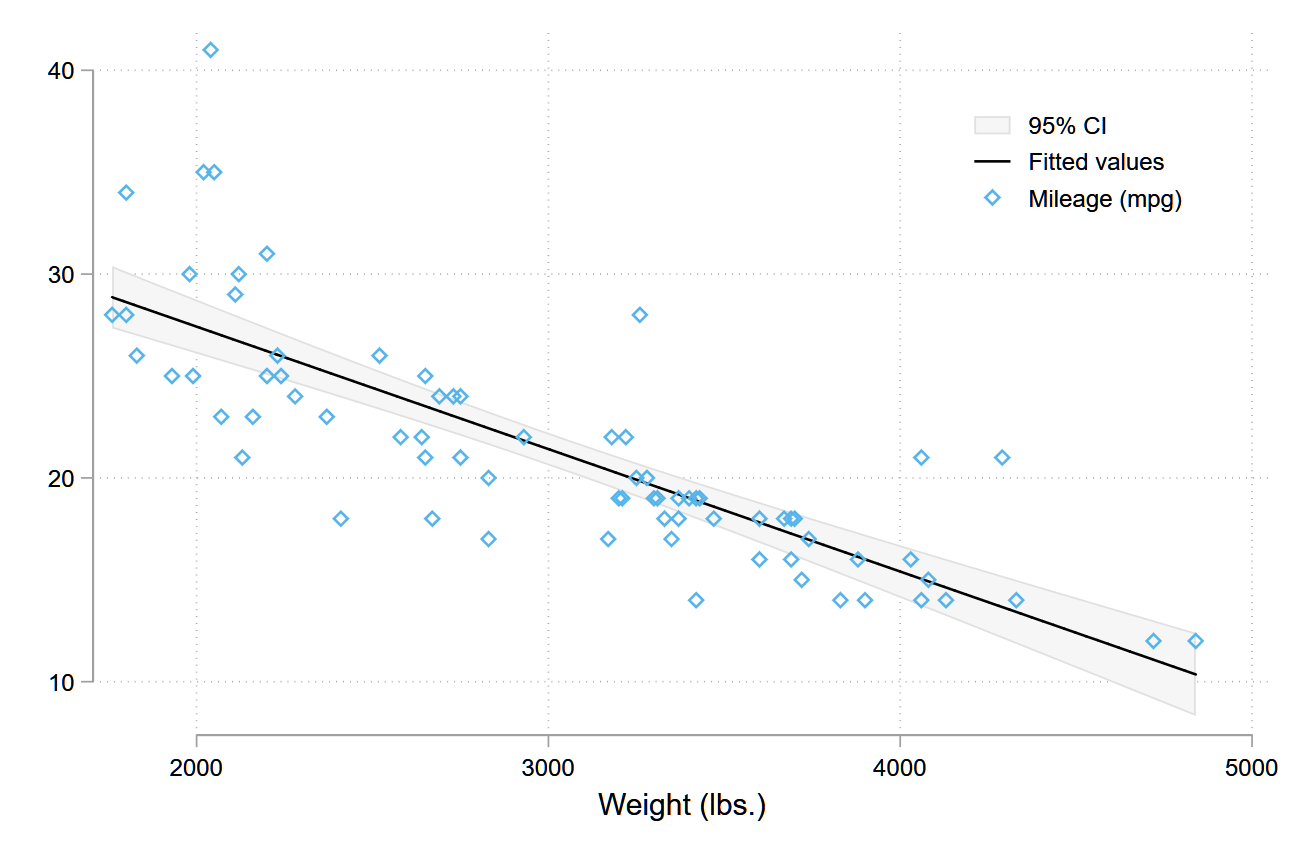
\includegraphics[width=0.6\textwidth]{mpg.png}
	\caption{Scatter Plot: MPG V.S. Weight\label{fig:mpg}}
\end{figure}
	
	

考虑函数 $y=a+bx$, 其中 $a$ 和 $b$ 是待定常数。如果离散点完全的在一直线上,可以认为变量之间的关系为一元函数。但一般说来,这些点不可能在同一直线上。但是它只能用直线来描述时,计算值与实际值会产生偏差。当然要求偏差越小越好,但由于偏差可正可负,因此不能认为总偏差时,拟合函数很好地反映了变量之间的关系,但是因为此时每个偏差的绝对值可能很大。为了改进这一缺陷,就考虑用平均值来代替。但是由于绝对值不易作解析运算,因此,进一步用残差平方和函数来度量总偏差。偏差的平方和最小可以保证每个偏差都不会很大。于是问题归结为确定拟合函数中的常数和使残差平方和函数最小。 

	

\begin{table}[!htbp]
  \small
  \centering
  \caption{Regression Result Example}
    \begin{tabular}{lll}
    \toprule
          & \multicolumn{1}{c}{(1)} & \multicolumn{1}{c}{(2)} \\
      & \multicolumn{1}{c}{price} & \multicolumn{1}{c}{price} \\
    \midrule
    mpg   & \multicolumn{1}{c}{-238.9***} & \multicolumn{1}{c}{-49.51} \\
          & \multicolumn{1}{c}{(53.08)} & \multicolumn{1}{c}{(86.16)} \\
    weight & \multicolumn{1}{c}{} & \multicolumn{1}{c}{1.747***} \\
          & \multicolumn{1}{c}{} & \multicolumn{1}{c}{(0.641)} \\
    constant & \multicolumn{1}{c}{11,253***} & \multicolumn{1}{c}{1,946} \\
          & \multicolumn{1}{c}{(1,171)} & \multicolumn{1}{c}{(3,597)} \\
    observations & \multicolumn{1}{c}{74} & \multicolumn{1}{c}{74} \\
    R-squared & \multicolumn{1}{c}{0.220} & \multicolumn{1}{c}{0.293} \\
    \midrule
    \multicolumn{3}{l}{\scriptsize Standard errors in parentheses} \\
    \multicolumn{3}{l}{\scriptsize *** p<0.01, ** p<0.05, * p<0.1} \\
    \end{tabular}%
  \label{tab:reg}%
\end{table}%


\begin{itemize}[noitemsep]
	\item Routing and resource discovery;
	     \begin{itemize} 
      	   	\item Language Models
       	 	\item Vector Space Models
    		 \end{itemize}
	\item Resilient and scalable computer networks;
	\item Distributed storage and search.
\end{itemize}



\end{document}
